\section{Weryfikacja}

\paragraph{Wskazanie popularności elementów}
Przegląd map cieplnych pozwala na łatwą identyfikację częściej i rzadziej używanych funkcji, ekranów i elementów interfejsu. Szczególnie dobrze nadają się do tego celu mapy kumulacyjne elementów nawigacji. Testowana aplikacja posiada dolny pasek nawigacji dzielący ją na trzy obszary: Panel, Plany oraz Nagrody. Na poniższej mapie można łatwo zauważyć że pierwsza zakładka jest używana najczęściej a pozostałe dwie są wybierane w przybliżeniu tak samo często.

\bigskip
\img{\chapterPath/[bottom-nav-bar].png}{Pasek nawigacji testowanej aplikacji}{rs_bottom_nav_bar}{.7}

\paragraph{Ekrany i obszary przewijane}
Ekrany posiadające potencjalnie przewijane obszary muszą być rozdzielone na mapę interakcji ze statycznymi elementami interfejsu oraz z zawartością znajdującą się w przewijanym polu. Na poniższych obrazkach przedstawiony jest przykład takiej sytuacji. Po prawej stronie znajduje się mapa obszaru przewiniętego przez użytkownika. Widać też miejsca w których dotykał on ekranu podczas tej czynności. 

\bigskip
\begin{figure}[H]
\centering
\begin{minipage}{.35\textwidth}
	\centering
	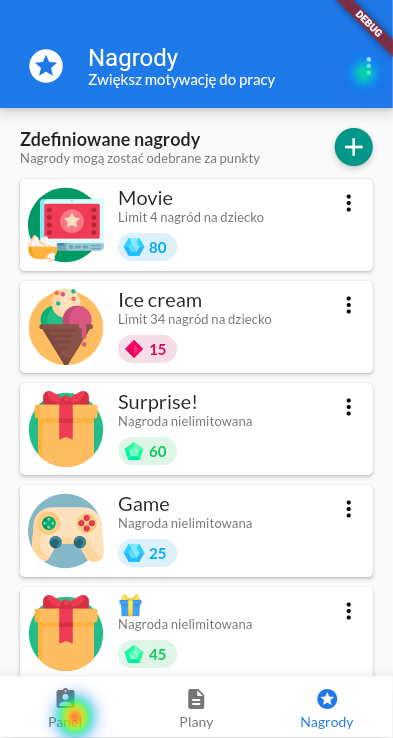
\includegraphics[width=.9\linewidth]{\chapterPath/caregiver-awards-page.png}
\end{minipage}
\begin{minipage}{.35\textwidth}
	\centering
	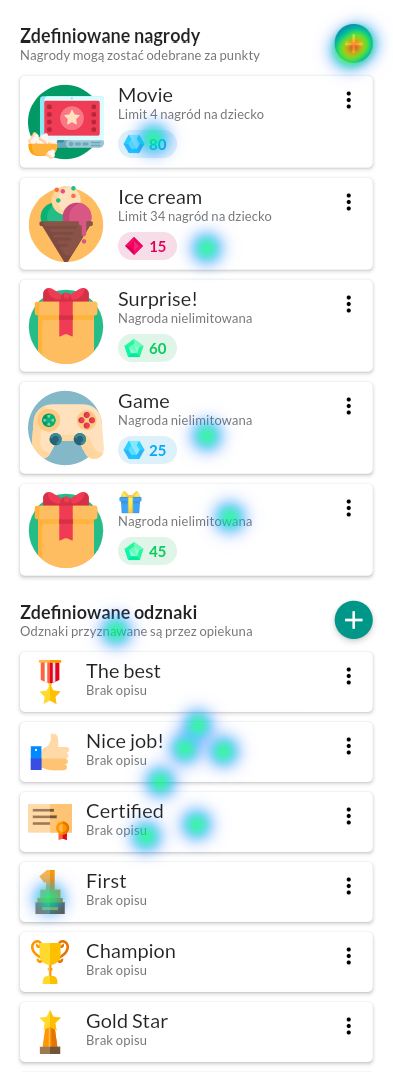
\includegraphics[width=.9\linewidth]{\chapterPath/[main-scroll-area] caregiver-awards-page.png}
\end{minipage}
\bigskip
\caption{Ekran nagród użytkownika}
\label{fig:rs_panel_parts}
\end{figure}

\paragraph{Niewidoczne elementy}


\paragraph{Zmienne elementy}
W przypadku przewijanych obszarów zawierających animowane (zmieniające wielkość, kształt lub zawartość) elementy, tło stworzonych map może nie być spójne. Wynika to z opisanego już mechanizmu stopniowego tworzenia tła z części wyświetlanych na ekranie w danym momencie. W poniższym przykładzie po lewej stronie widać widok kart na ekranie aplikacji. W trakcie przewijania widok jest animowany powodując powiększenie aktualnie wyświetlanej na środku karty. Po lewej umieszczona została mapa cieplna złożona z trzech kart po ich przewinięciu przez użytkownika. Z powodu połączenia obrazków na których ta sama karta ma różną wielkość obie boczne karty zawierają defekty graficzne. Pomimo tego ograniczenia wynikowe tło mapy cieplnej nadal spełnia swoją funkcję pozwalając na umiejscowienie interakcji użytkowników w stosunku do elementów interfejsu.

\bigskip
\begin{figure}[H]
\begin{minipage}{.25\textwidth}
	\centering
	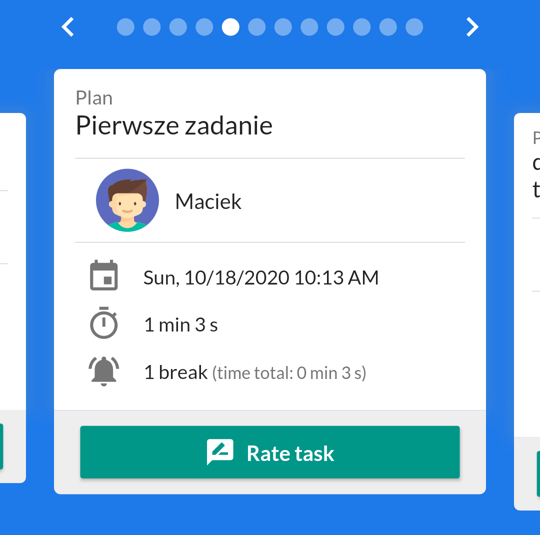
\includegraphics[width=.9\linewidth]{\chapterPath/rating_cards-app.png}
\end{minipage}
\begin{minipage}{.74\textwidth}
	\centering
	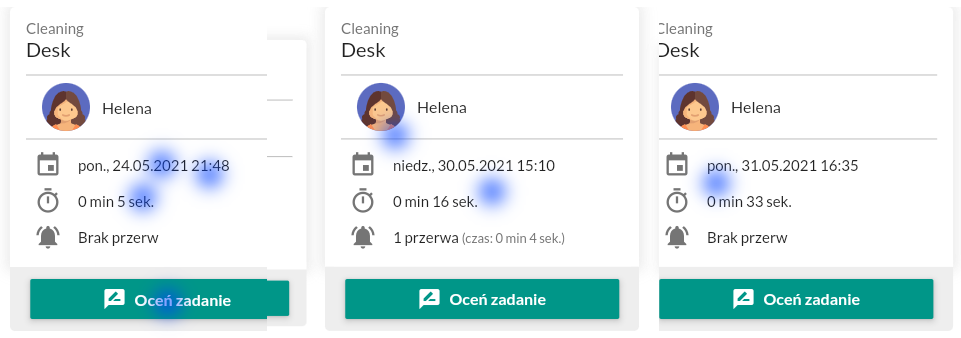
\includegraphics[width=.9\linewidth]{\chapterPath/[rating-cards]-caregiver-rating-page.png}
\end{minipage}
\bigskip
\caption{Widok kart w aplikacji oraz na mapie cieplnej}
\label{fig:rs_rating_cards}
\end{figure}
